\documentclass[12pt,a4paper,openany,twoside]{ctexbook}
%-------------------------------------宏包引用---------------------------------------------------
\usepackage[paperwidth=185mm,paperheight=230mm,textheight=190mm,textwidth=145mm,left=20mm,right=20mm, top=25mm, bottom=15mm]{geometry}            %定义版面
%--------------------------------------------------------------------------------------
\usepackage{fontspec}
\usepackage{xunicode}
\usepackage{xltxtra}
%--------------------------------------------------------------------------------------
\usepackage[listings,theorems]{tcolorbox}
\usepackage{fancybox}                 % 边框,有阴影,fancybox提供了五种式样\fbox,\shadowbox,\doublebox,\ovalbox,\Ovalbox。
\usepackage{colortbl}                   % 单元格加背景
\usepackage{fancyhdr}                 % 页眉和页脚的相关定义
\usepackage[CJKbookmarks, colorlinks, bookmarksnumbered=true,pdfstartview=FitH,linkcolor=black]{hyperref}   % 书签功能,选项去掉链接红色方框
\usepackage{mathtools}
\usepackage{amssymb}
\usepackage{bm}	% 处理数学公式中的黑斜体的宏包

\usepackage{subfigure}

\usepackage{algorithm}
\usepackage{algorithmic}

\usepackage[amsmath,thmmarks]{ntheorem}         % 定理类环境宏包,其中 amsmath 选项用来兼容 AMS LaTeX 的宏包thmmarks 选项,可以自动恰当地放置定理类环境的结束标记;它还能像图形目录那样生成定理类环境目录

\usepackage{fancyref}                                % 支持引用的宏包   %引用宏包所在位置
%-----------------------------------------------------主文档 格式定义---------------------------------
\addtolength{\headsep}{-0.1cm}        %页眉位置
%\addtolength{\footskip}{0.4cm}       %页脚位置
%-----------------------------------------------------设定字体等------------------------------
\setmainfont{Times New Roman}    % 缺省字体
%\setCJKfamilyfont{song}{SimSun}
%\setCJKfamilyfont{hei}{SimHei}
%\setCJKfamilyfont{kai}{KaiTi}
%\setCJKfamilyfont{fs}{FangSong}
%\setCJKfamilyfont{li}{LiSu}
%\setCJKfamilyfont{you}{YouYuan}
%\setCJKfamilyfont{yahei}{Microsoft YaHei}
%\setCJKfamilyfont{xingkai}{STXingkai}
%\setCJKfamilyfont{xinwei}{STXinwei}
%\setCJKfamilyfont{fzyao}{FZYaoTi}
%\setCJKfamilyfont{fzshu}{FZShuTi}
%-------------------------------------------------------------------
\newCJKfontfamily\song{SimSun}
\newCJKfontfamily\hei{SimHei}
\newCJKfontfamily\kai{KaiTi}
\newCJKfontfamily\fs{FangSong}
\newCJKfontfamily\li{LiSu}
\newCJKfontfamily\you{YouYuan}
%\newCJKfontfamily\yahei{Microsoft YaHei}
\newCJKfontfamily\xingkai{STXingkai}
\newCJKfontfamily\xinwei{STXinwei}
\newCJKfontfamily\fzyao{FZYaoTi}
\newCJKfontfamily\fzshu{FZShuTi}
%------------------------------------------------------------------------------------------------------
\newcommand{\linghao}{\fontsize{48pt}{60pt}\selectfont}      % 零号, 1.4倍行距
\newcommand{\chuhao}{\fontsize{42pt}{\baselineskip}\selectfont}  % 初号& 42pt
\newcommand{\xiaochuhao}{\fontsize{36pt}{\baselineskip}\selectfont} % 小初号& 36pt
\newcommand{\yihao}{\fontsize{28pt}{38pt}\selectfont}        % 一号, 1.4倍行距
\newcommand{\erhao}{\fontsize{21pt}{28pt}\selectfont}        % 二号, 1.25倍行距
\newcommand{\xiaoer}{\fontsize{18pt}{18pt}\selectfont}       % 小二, 单倍行距
\newcommand{\sanhao}{\fontsize{16pt}{24pt}\selectfont}       % 三号, 1.5倍行距
\newcommand{\xiaosan}{\fontsize{15pt}{22pt}\selectfont}      % 小三, 1.5倍行距
\newcommand{\sihao}{\fontsize{14pt}{21pt}\selectfont}        % 四号, 1.5倍行距
\newcommand{\xiaosihao}{\fontsize{12pt}{18pt}\selectfont}    % 小四, 1.5倍行距
\newcommand{\dawuhao}{\fontsize{11pt}{11pt}\selectfont}      % 大五号, 单倍行距
\newcommand{\wuhao}{\fontsize{10.5pt}{10.5pt}\selectfont}    % 五号, 单倍行距
\newcommand{\xiaowuhao}{\fontsize{10pt}{10pt}\selectfont}    % 小五号, 单倍行距
\newcommand{\liuhao}{\fontsize{7.875pt}{7.875pt}\selectfont} % 六号, 单倍行距
\newcommand{\qihao}{\fontsize{5.25pt}{\baselineskip}\selectfont}
%--------------------------------------------------------------------------------------------------------
%-----------------------------------------------------------定义颜色---------------
\definecolor{blueblack}{cmyk}{0,0,0,0.35}%浅黑
\definecolor{darkblue}{cmyk}{1,0,0,0}%纯蓝
\definecolor{lightblue}{cmyk}{0.15,0,0,0}%浅蓝
%--------------------------------------------------------设定标题颜色--------------
\CTEXsetup[format+={\li \color{black}}]{chapter}
\CTEXsetup[format+={\li \color{black}}]{section}
\CTEXsetup[format+={\li \color{black}}]{subsection}

%-----------重定义带编号标题----------------------------
\theoremstyle{plain}
\theoremheaderfont{\hei\rmfamily}
\theorembodyfont{\song\rmfamily}
\theoremseparator{~}%帽号 : 改为 ~ 变空格
\newtheorem{block}{\indent\color{darkblue}}
\newtheorem{definition}{\indent\color{darkblue}定义}[section]
\newtheorem{proposition}{\indent\color{darkblue}命题}[section]
\newtheorem{theorem}{\indent\color{darkblue}定理}[section]
\newtheorem{lemma}{\indent\color{darkblue}引理}[section]
\newtheorem{axiom}{\indent\color{darkblue}公理}[section]
\newtheorem{corollary}{\indent\color{darkblue}推论}[section]
\newtheorem{character}{\indent\color{darkblue}性质}[section]


\newtheorem{exam}{\indent\hei \color{darkblue}例}[chapter]
\newtheorem{exercise}{\indent\hei \color{darkblue}题}
\newtheorem{example}{\hspace{2em}\hei\color{white}Matlab程序}[section]
\newcommand{\program}[1]{\noindent\parbox{14.6cm}{\includegraphics[width=3.1cm]{fig/sjwt.jpg}
		\vspace{-1.12cm}\example\textcolor{darkblue}{\hei#1}}\vspace{0.0cm}}  %实际问题标志



%------------------------------------------重定义不带编号标题----------------------------
\theoremstyle{nonumberplain} \theoremseparator{~}    %帽号 : 改为 ~ 变空格
%\theoremsymbol{$\blacksquare$}                      %在证明结束行尾加上一个黑色方块
\newtheorem{proof}{\indent\hei \textcolor{darkblue}{证明}}
\newtheorem{Solution}{\indent\hei \textcolor{darkblue}{解}}
\newtheorem{REFERENCE}{\indent\hei\sihao \textcolor{darkblue}{参考文献}}
%==========程序框====================================
\newcommand{\programbox}[2]{
	\begin{tcolorbox}[colback=white,colframe=darkblue,title=\example #1]
		#2
\end{tcolorbox}}
%==========程序框结束====================================

%==========命题框====================================
\newcommand{\propositionbox}[1]{\vspace{0.3cm}
	\begin{colorboxed}[boxcolor=darkblue,bgcolor=white]
		\vspace{-0.3cm}\proposition #1
\end{colorboxed}}
%==========命题框结束====================================

%==========引理框====================================
\newcommand{\lemmabox}[1]{\vspace{0.3cm}
	\begin{colorboxed}[boxcolor=darkblue,bgcolor=white]
		\vspace{-0.3cm}\lemma #1
\end{colorboxed}}
%==========引理框结束====================================

%==========定理框====================================
\newcommand{\theorebox}[1]{\vspace{0.3cm}
	\begin{colorboxed}[boxcolor=darkblue,bgcolor=lightblue]
		\vspace{-0.3cm}\theorem #1
\end{colorboxed}}
%==========定理框结束====================================

%==========推论框====================================
\newcommand{\corolbox}[1]{\vspace{0.3cm}
	\begin{colorboxed}[boxcolor=darkblue,bgcolor=white]
		\vspace{-0.3cm}\corollary #1
\end{colorboxed}}
%==========推论框结束====================================

%==========性质框====================================
\newcommand{\charactbox}[1]{\vspace{0.3cm}
	\begin{colorboxed}[boxcolor=darkblue,bgcolor=white]
		\vspace{-0.3cm}\character #1
\end{colorboxed}}
%==========性质框结束====================================

%==========定义框====================================
\newcommand{\definibox}[2]{\vspace{0.3cm}
	\begin{colorboxed}[boxcolor=darkblue,fgcolor=white,bgcolor=darkblue]
		\vspace{-0.4cm}
		\definition\hei\color{white}#1
		\vspace{0.04cm}
	\end{colorboxed}
	\vspace{-0.7cm} \setlength{\fboxsep}{4pt}
	\begin{colorboxed}[boxcolor=darkblue,fgcolor=black,bgcolor=lightblue]
		#2
	\end{colorboxed}\color{black}}
%==========定义框结束====================================

%%-----------------------------------------------------------定义、定理环境-------------------------
%\newcounter{myDefinition}[chapter]\def\themyDefinition{\thechapter.\arabic{myDefinition}}
%\newcounter{myTheorem}[chapter]\def\themyTheorem{\thechapter.\arabic{myTheorem}}
%\newcounter{myCorollary}[chapter]\def\themyCorollary{\thechapter.\arabic{myCorollary}}
%
%\tcbmaketheorem{defi}{定义}{fonttitle=\bfseries\upshape, fontupper=\slshape, arc=0mm, colback=lightblue,colframe=darkblue}{myDefinition}{Definition}
%\tcbmaketheorem{theo}{定理}{fonttitle=\bfseries\upshape, fontupper=\slshape, arc=0mm, colback=lightblue,colframe=darkblue}{myTheorem}{Theorem}
%\tcbmaketheorem{coro}{推论}{fonttitle=\bfseries\upshape, fontupper=\slshape, arc=0mm, colback=lightblue,colframe=darkblue}{myCorollary}{Corollary}
%%------------------------------------------------------------------------------
%\newtheorem{proof}{\indent\hei \textcolor{darkblue}{证明}}
%\newtheorem{Solution}{\indent\hei \textcolor{darkblue}{解}}
%------------------------------------------------定义页眉下单隔线----------------
\newcommand{\makeheadrule}{\makebox[0pt][l]{\color{darkblue}\rule[.7\baselineskip]{\headwidth}{0.3pt}}\vskip-.8\baselineskip}
%-----------------------------------------------定义页眉下双隔线----------------
\makeatletter
\renewcommand{\headrule}{{\if@fancyplain\let\headrulewidth\plainheadrulewidth\fi\makeheadrule}}
\pagestyle{fancy}
\renewcommand{\chaptermark}[1]{\markboth{第\chaptername 章\quad #1}{}}    %去掉章标题中的数字
\renewcommand{\sectionmark}[1]{\markright{\thesection\quad #1}{}}    %去掉节标题中的点
\fancyhf{} %清空页眉
\fancyhead[RO]{\kai{\footnotesize.~\color{darkblue}\thepage~.}}         % 奇数页码显示左边
\fancyhead[LE]{\kai{\footnotesize.~\color{darkblue}\thepage~.}}         % 偶数页码显示右边
\fancyhead[CO]{\song\footnotesize\color{darkblue}\rightmark} % 奇数页码中间显示节标题
\fancyhead[CE]{\song\footnotesize\color{darkblue}\leftmark}  % 偶数页码中间显示章标题
%---------------------------------------------------------------------------------------------------------------------


    %格式所在位置
% !Mode:: "TeX:UTF-8"
\newcommand{\normmm}[1]{{\left\vert\kern-0.25ex\left\vert\kern-0.25ex\left\vert #1 
		\right\vert\kern-0.25ex\right\vert\kern-0.25ex\right\vert}}

\newcommand{\argmax}{\arg\max}
\newcommand{\argmin}{\arg\min}
\newcommand{\sigmoid}{\text{sigmoid}}
\newcommand{\norm}[1]{\left\lVert#1\right\rVert}
\newcommand{\inprod}[2]{\langle#1,#2\rangle}
\newcommand{\Tr}{\text{Tr}}
\renewcommand{\d}{\text{d}}

\newcommand{\Var}{\text{Var}}
\newcommand{\Cov}{\text{Cov}}
\newcommand{\plim}{\text{plim}}
\newcommand{\Tsp}{\top}

\newcommand{\diag}{\mathop{\rm diag}\nolimits}
\newcommand{\rank}{\mathop{\rm rank}\nolimits}
\newcommand{\Laplace}{\mathop{\rm Laplace}\nolimits}
\newcommand{\Bernoulli}{\mathop{\rm Bernoulli}\nolimits}
\newcommand{\Uniform}{\mathop{\rm Uniform}\nolimits}
\newcommand{\Possion}{\mathop{\rm Possion}\nolimits}
\newcommand{\Ber}{\mathop{\rm Ber}\nolimits}
\newcommand{\Bin}{\mathop{\rm Bin}\nolimits}
\newcommand{\Cat}{\mathop{\rm Cat}\nolimits}
\newcommand{\Dir}{\mathop{\rm Dir}\nolimits}
\newcommand{\Lap}{\mathop{\rm Lap}\nolimits}
\newcommand{\sigm}{\mathop{\rm sigm}\nolimits}

\newcommand{\RSS}{\mathop{\rm RSS}\nolimits}
\newcommand{\se}{\mathop{\rm se}\nolimits}
\newcommand{\logit}{\mathop{\rm logit}\nolimits}
\newcommand{\dom}{\mathop{\bf dom}\nolimits}
\newcommand{\epi}{\mathop{\bf epi}\nolimits}
\newcommand{\hypo}{\mathop{\bf hypo}\nolimits}
\newcommand{\prob}{\mathop{\bf prob}\nolimits}
\newcommand{\relint}{\mathop{\bf relint}\nolimits}
\newcommand{\aff}{\mathop{\bf aff}\nolimits}
\newcommand{\spn}{\mathop{\bf span}\nolimits}
% Scala 标量 暂不使用
\newcommand{\Sa}{\mathit{a}}
\newcommand{\Sb}{\mathit{b}}
\newcommand{\Sc}{\mathit{c}}
\newcommand{\Sd}{\mathit{d}}
\newcommand{\Se}{\mathit{e}}
\newcommand{\Sf}{\mathit{f}}
\newcommand{\Sg}{\mathit{g}}
\newcommand{\Sh}{\mathit{h}}
\newcommand{\Si}{\mathit{i}}
\newcommand{\Sj}{\mathit{j}}
\newcommand{\Sk}{\mathit{k}}
\newcommand{\Sl}{\mathit{l}}
\newcommand{\Sm}{\mathit{m}}
\newcommand{\Sn}{\mathit{n}}
\newcommand{\So}{\mathit{o}}
\newcommand{\Sp}{\mathit{p}}
\newcommand{\Sq}{\mathit{q}}
\newcommand{\Sr}{\mathit{r}}
\newcommand{\Ss}{\mathit{s}}
\newcommand{\St}{\mathit{t}}
\newcommand{\Su}{\mathit{u}}
\newcommand{\Sv}{\mathit{v}}
\newcommand{\Sw}{\mathit{w}}
\newcommand{\Sx}{\mathit{x}}
\newcommand{\Sy}{\mathit{y}}
\newcommand{\Sz}{\mathit{z}}

\newcommand{\SA}{\mathit{A}}
\newcommand{\SB}{\mathit{B}}
\newcommand{\SC}{\mathit{C}}
\newcommand{\SD}{\mathit{D}}
\newcommand{\SE}{\mathit{E}}
\newcommand{\SF}{\mathit{F}}
\newcommand{\SG}{\mathit{G}}
\newcommand{\SH}{\mathit{H}}
\newcommand{\SJ}{\mathit{J}}
\newcommand{\SK}{\mathit{K}}
\newcommand{\SI}{\mathit{L}}
\newcommand{\SM}{\mathit{M}}
\newcommand{\SN}{\mathit{N}}
\newcommand{\SO}{\mathit{O}}
\newcommand{\SP}{\mathit{P}}
\newcommand{\SQ}{\mathit{Q}}
\newcommand{\SR}{\mathit{R}}
\newcommand{\ST}{\mathit{T}}
\newcommand{\SU}{\mathit{U}}
\newcommand{\SV}{\mathit{V}}
\newcommand{\SW}{\mathit{W}}
\newcommand{\SX}{\mathit{X}}
\newcommand{\SY}{\mathit{Y}}
\newcommand{\SZ}{\mathit{Z}}



% Vector 向量 \VI 全1向量 \VO 零向量
\newcommand{\Va}{\boldsymbol{\mathit{a}}}
\newcommand{\Vb}{\boldsymbol{\mathit{b}}}
\newcommand{\Vc}{\boldsymbol{\mathit{c}}}
\newcommand{\Vd}{\boldsymbol{\mathit{d}}}
\newcommand{\Ve}{\boldsymbol{\mathit{e}}}
\newcommand{\Vf}{\boldsymbol{\mathit{f}}}
\newcommand{\Vg}{\boldsymbol{\mathit{g}}}
\newcommand{\Vh}{\boldsymbol{\mathit{h}}}
\newcommand{\Vi}{\boldsymbol{\mathit{i}}}
\newcommand{\Vj}{\boldsymbol{\mathit{j}}}
\newcommand{\Vk}{\boldsymbol{\mathit{k}}}
\newcommand{\Vl}{\boldsymbol{\mathit{l}}}
\newcommand{\Vm}{\boldsymbol{\mathit{m}}}
\newcommand{\Vn}{\boldsymbol{\mathit{n}}}
\newcommand{\Vo}{\boldsymbol{\mathit{o}}}
\newcommand{\Vp}{\boldsymbol{\mathit{p}}}
\newcommand{\Vq}{\boldsymbol{\mathit{q}}}
\newcommand{\Vr}{\boldsymbol{\mathit{r}}}
\newcommand{\Vs}{\boldsymbol{\mathit{s}}}
\newcommand{\Vt}{\boldsymbol{\mathit{t}}}
\newcommand{\Vu}{\boldsymbol{\mathit{u}}}
\newcommand{\Vv}{\boldsymbol{\mathit{v}}}
\newcommand{\Vw}{\boldsymbol{\mathit{w}}}
\newcommand{\Vx}{\boldsymbol{\mathit{x}}}
\newcommand{\Vy}{\boldsymbol{\mathit{y}}}
\newcommand{\Vz}{\boldsymbol{\mathit{z}}}

%零向量,由于命令中不能出现数字,用字母“O”代替数字“0”
\newcommand{\VO}{\boldsymbol{0}}
\newcommand{\VI}{\boldsymbol{1}}

% Matrix 矩阵
\newcommand{\MA}{\boldsymbol{\mathit{A}}}
\newcommand{\MB}{\boldsymbol{\mathit{B}}}
\newcommand{\MC}{\boldsymbol{\mathit{C}}}
\newcommand{\MD}{\boldsymbol{\mathit{D}}}
\newcommand{\ME}{\boldsymbol{\mathit{E}}}
\newcommand{\MF}{\boldsymbol{\mathit{F}}}
\newcommand{\MG}{\boldsymbol{\mathit{G}}}
\newcommand{\MH}{\boldsymbol{\mathit{H}}}
\newcommand{\MI}{\boldsymbol{\mathit{I}}}
\newcommand{\MJ}{\boldsymbol{\mathit{J}}}
\newcommand{\MK}{\boldsymbol{\mathit{K}}}
\newcommand{\ML}{\boldsymbol{\mathit{L}}}
\newcommand{\MM}{\boldsymbol{\mathit{M}}}
\newcommand{\MN}{\boldsymbol{\mathit{N}}}
\newcommand{\MO}{\boldsymbol{\mathit{O}}}
\newcommand{\MP}{\boldsymbol{\mathit{P}}}
\newcommand{\MQ}{\boldsymbol{\mathit{Q}}}
\newcommand{\MR}{\boldsymbol{\mathit{R}}}
\newcommand{\MS}{\boldsymbol{\mathit{S}}}
\newcommand{\MT}{\boldsymbol{\mathit{T}}}
\newcommand{\MU}{\boldsymbol{\mathit{U}}}
\newcommand{\MV}{\boldsymbol{\mathit{V}}}
\newcommand{\MW}{\boldsymbol{\mathit{W}}}
\newcommand{\MX}{\boldsymbol{\mathit{X}}}
\newcommand{\MY}{\boldsymbol{\mathit{Y}}}
\newcommand{\MZ}{\boldsymbol{\mathit{Z}}}


%Tensor 张量
\newcommand{\TSA}{\textsf{\textbf{A}}}
\newcommand{\TSB}{\textsf{\textbf{B}}}
\newcommand{\TSC}{\textsf{\textbf{C}}}
\newcommand{\TSD}{\textsf{\textbf{D}}}
\newcommand{\TSE}{\textsf{\textbf{E}}}
\newcommand{\TSF}{\textsf{\textbf{F}}}
\newcommand{\TSG}{\textsf{\textbf{G}}}
\newcommand{\TSH}{\textsf{\textbf{H}}}
\newcommand{\TSI}{\textsf{\textbf{I}}}
\newcommand{\TSJ}{\textsf{\textbf{J}}}
\newcommand{\TSK}{\textsf{\textbf{K}}}
\newcommand{\TSL}{\textsf{\textbf{L}}}
\newcommand{\TSM}{\textsf{\textbf{M}}}
\newcommand{\TSN}{\textsf{\textbf{N}}}
\newcommand{\TSO}{\textsf{\textbf{O}}}
\newcommand{\TSP}{\textsf{\textbf{P}}}
\newcommand{\TSQ}{\textsf{\textbf{Q}}}
\newcommand{\TSR}{\textsf{\textbf{R}}}
\newcommand{\TSS}{\textsf{\textbf{S}}}
\newcommand{\TST}{\textsf{\textbf{T}}}
\newcommand{\TSU}{\textsf{\textbf{U}}}
\newcommand{\TSV}{\textsf{\textbf{V}}}
\newcommand{\TSW}{\textsf{\textbf{W}}}
\newcommand{\TSX}{\textsf{\textbf{X}}}
\newcommand{\TSY}{\textsf{\textbf{Y}}}
\newcommand{\TSZ}{\textsf{\textbf{Z}}}

% Tensor Element
\newcommand{\TEA}{\textit{\textsf{A}}}
\newcommand{\TEB}{\textit{\textsf{B}}}
\newcommand{\TEC}{\textit{\textsf{C}}}
\newcommand{\TED}{\textit{\textsf{D}}}
\newcommand{\TEE}{\textit{\textsf{E}}}
\newcommand{\TEF}{\textit{\textsf{F}}}
\newcommand{\TEG}{\textit{\textsf{G}}}
\newcommand{\TEH}{\textit{\textsf{H}}}
\newcommand{\TEI}{\textit{\textsf{I}}}
\newcommand{\TEJ}{\textit{\textsf{J}}}
\newcommand{\TEK}{\textit{\textsf{K}}}
\newcommand{\TEL}{\textit{\textsf{L}}}
\newcommand{\TEM}{\textit{\textsf{M}}}
\newcommand{\TEN}{\textit{\textsf{N}}}
\newcommand{\TEO}{\textit{\textsf{O}}}
\newcommand{\TEP}{\textit{\textsf{P}}}
\newcommand{\TEQ}{\textit{\textsf{Q}}}
\newcommand{\TER}{\textit{\textsf{R}}}
\newcommand{\TES}{\textit{\textsf{S}}}
\newcommand{\TET}{\textit{\textsf{T}}}
\newcommand{\TEU}{\textit{\textsf{U}}}
\newcommand{\TEV}{\textit{\textsf{V}}}
\newcommand{\TEW}{\textit{\textsf{W}}}
\newcommand{\TEX}{\textit{\textsf{X}}}
\newcommand{\TEY}{\textit{\textsf{Y}}}
\newcommand{\TEZ}{\textit{\textsf{Z}}}

% Random Scala
\newcommand{\RSa}{\mathrm{a}}
\newcommand{\RSb}{\mathrm{b}}
\newcommand{\RSc}{\mathrm{c}}
\newcommand{\RSd}{\mathrm{d}}
\newcommand{\RSe}{\mathrm{e}}
\newcommand{\RSf}{\mathrm{f}}
\newcommand{\RSg}{\mathrm{g}}
\newcommand{\RSh}{\mathrm{h}}
\newcommand{\RSi}{\mathrm{i}}
\newcommand{\RSj}{\mathrm{j}}
\newcommand{\RSk}{\mathrm{k}}
\newcommand{\RSl}{\mathrm{l}}
\newcommand{\RSm}{\mathrm{m}}
\newcommand{\RSn}{\mathrm{n}}
\newcommand{\RSo}{\mathrm{o}}
\newcommand{\RSp}{\mathrm{p}}
\newcommand{\RSq}{\mathrm{q}}
\newcommand{\RSr}{\mathrm{r}}
\newcommand{\RSs}{\mathrm{s}}
\newcommand{\RSt}{\mathrm{t}}
\newcommand{\RSu}{\mathrm{u}}
\newcommand{\RSv}{\mathrm{v}}
\newcommand{\RSw}{\mathrm{w}}
\newcommand{\RSx}{\mathrm{x}}
\newcommand{\RSy}{\mathrm{y}}
\newcommand{\RSz}{\mathrm{z}}


% Random Vector
\newcommand{\RVa}{\mathbf{a}}
\newcommand{\RVb}{\mathbf{b}}
\newcommand{\RVc}{\mathbf{c}}
\newcommand{\RVd}{\mathbf{d}}
\newcommand{\RVe}{\mathbf{e}}
\newcommand{\RVf}{\mathbf{f}}
\newcommand{\RVg}{\mathbf{g}}
\newcommand{\RVh}{\mathbf{h}}
\newcommand{\RVi}{\mathbf{i}}
\newcommand{\RVj}{\mathbf{j}}
\newcommand{\RVk}{\mathbf{k}}
\newcommand{\RVl}{\mathbf{l}}
\newcommand{\RVm}{\mathbf{m}}
\newcommand{\RVn}{\mathbf{n}}
\newcommand{\RVo}{\mathbf{o}}
\newcommand{\RVp}{\mathbf{p}}
\newcommand{\RVq}{\mathbf{q}}
\newcommand{\RVr}{\mathbf{r}}
\newcommand{\RVs}{\mathbf{s}}
\newcommand{\RVt}{\mathbf{t}}
\newcommand{\RVu}{\mathbf{u}}
\newcommand{\RVv}{\mathbf{v}}
\newcommand{\RVw}{\mathbf{w}}
\newcommand{\RVx}{\mathbf{x}}
\newcommand{\RVy}{\mathbf{y}}
\newcommand{\RVz}{\mathbf{z}}

% Random Matrix
\newcommand{\RMX}{\boldsymbol{\mathrm{X}}}
\newcommand{\RMA}{\boldsymbol{\mathrm{A}}}

\newcommand{\Valpha}{\boldsymbol{\alpha}}
\newcommand{\Vbeta}{\boldsymbol{\beta}}
\newcommand{\Vtheta}{\boldsymbol{\theta}}
\newcommand{\Vlambda}{\boldsymbol{\lambda}}
\newcommand{\Veta}{\boldsymbol{\eta}}
\newcommand{\Vepsilon}{\boldsymbol{\varepsilon}}
\newcommand{\Vmu}{\boldsymbol{\mu}}
\newcommand{\VPhi}{\boldsymbol{\Phi}}
\newcommand{\Vsigma}{\boldsymbol{\sigma}}

\newcommand{\Vrho}{\boldsymbol{\rho}}
\newcommand{\Vgamma}{\boldsymbol{\gamma}}
\newcommand{\Vomega}{\boldsymbol{\omega}}
\newcommand{\Vpsi}{\boldsymbol{\psi}}
\newcommand{\Vzeta}{\boldsymbol{\zeta}}
\newcommand{\Vxi}{\boldsymbol{\xi}}
\newcommand{\Vone}{\boldsymbol{1}}
\newcommand{\Vvarphi}{\boldsymbol{\varphi}}
\newcommand{\MLambda}{\boldsymbol{\Lambda}}
\newcommand{\MSigma}{\boldsymbol{\Sigma}}

\newcommand{\MPi}{\boldsymbol{\mathit{\Pi}}}

%线性变换 书法字体 \CalA
\newcommand{\CalA}{\mathcal{A}}
\newcommand{\CalB}{\mathcal{B}}
\newcommand{\CalC}{\mathcal{C}}
\newcommand{\CalD}{\mathcal{D}}
\newcommand{\CalE}{\mathcal{E}}
\newcommand{\CalF}{\mathcal{F}}
\newcommand{\CalG}{\mathcal{G}}
\newcommand{\CalH}{\mathcal{H}}
\newcommand{\CalI}{\mathcal{I}}
\newcommand{\CalJ}{\mathcal{J}}
\newcommand{\CalK}{\mathcal{K}}
\newcommand{\CalL}{\mathcal{L}}
\newcommand{\CalM}{\mathcal{M}}
\newcommand{\CalN}{\mathcal{N}}
\newcommand{\CalO}{\mathcal{O}}
\newcommand{\CalP}{\mathcal{P}}
\newcommand{\CalQ}{\mathcal{Q}}
\newcommand{\CalR}{\mathcal{R}}
\newcommand{\CalS}{\mathcal{S}}
\newcommand{\CalT}{\mathcal{T}}
\newcommand{\CalU}{\mathcal{U}}
\newcommand{\CalV}{\mathcal{V}}
\newcommand{\CalW}{\mathcal{W}}
\newcommand{\CalX}{\mathcal{X}}
\newcommand{\CalY}{\mathcal{Y}}
\newcommand{\CalZ}{\mathcal{Z}}


% Set
\newcommand{\SetA}{\mathbb{A}}
\newcommand{\SetB}{\mathbb{B}}
\newcommand{\SetC}{\mathbb{C}}
\newcommand{\SetD}{\mathbb{D}}
\newcommand{\SetE}{\mathbb{E}}
\newcommand{\SetF}{\mathbb{F}}
\newcommand{\SetG}{\mathbb{G}}
\newcommand{\SetH}{\mathbb{H}}
\newcommand{\SetI}{\mathbb{I}}
\newcommand{\SetJ}{\mathbb{J}}
\newcommand{\SetK}{\mathbb{K}}
\newcommand{\SetL}{\mathbb{L}}
\newcommand{\SetM}{\mathbb{M}}
\newcommand{\SetN}{\mathbb{N}}
\newcommand{\SetO}{\mathbb{O}}
\newcommand{\SetP}{\mathbb{P}}
\newcommand{\SetQ}{\mathbb{Q}}
\newcommand{\SetR}{\mathbb{R}}
\newcommand{\SetS}{\mathbb{S}}
\newcommand{\SetT}{\mathbb{T}}
\newcommand{\SetU}{\mathbb{U}}
\newcommand{\SetV}{\mathbb{V}}
\newcommand{\SetW}{\mathbb{W}}
\newcommand{\SetX}{\mathbb{X}}
\newcommand{\SetY}{\mathbb{Y}}
\newcommand{\SetZ}{\mathbb{Z}}


%Number Set
\newcommand{\NN}{\mathbb{N}}
\newcommand{\NZ}{\mathbb{Z}}
\newcommand{\NQ}{\mathbb{Q}}
\newcommand{\NR}{\mathbb{R}}
\newcommand{\NC}{\mathbb{C}}
\newcommand{\NK}{\mathbb{K}}

%转置
\renewcommand{\T}{^{\mathrm{T}}}


\newcommand{\Col}[1]{\text{Col}\left(#1\right)}
\newcommand{\Row}[1]{\text{Row}\left(#1\right)}
\newcommand{\Range}[1]{\text{Range}\left(#1\right)}
\newcommand{\Null}[1]{\text{Null}\left(#1\right)}
\newcommand{\nullity}[1]{\text{nullity}\left(#1\right)}
\newcommand{\Ker}[1]{\text{Ker}\left(#1\right)}
\let\olddefinition\definition
\let\oldproposition\proposition
\let\oldtheorem\theorem
\let\oldlemma\lemma
\let\oldaxiom\axiom
\let\oldcorollary\corollary
\let\oldcharacter\character
\let\oldexercise\exercise
\let\oldexam\exam
\let\oldexample\example

\let\oldequation\equation

%\renewcommand{\definition}{\olddefinition\label{dy:\thedefinition}}
%\renewcommand{\proposition}{\oldproposition\label{mt:\theproposition}}
%\renewcommand{\theorem}{\oldtheorem\label{dl:\thetheorem}}
%\renewcommand{\lemma}{\oldlemma\label{yl:\thelemma}}
%\renewcommand{\axiom}{\oldaxiom\label{gl:\theaxiom}}
%\renewcommand{\corollary}{\oldcorollary\label{tl:\thecorollary}}
%\renewcommand{\character}{\oldcharacter\label{xz:\thecharacter}}
%\renewcommand{\exercise}{\oldexercise\label{xt:\theexercise}}
%\renewcommand{\exam}{\oldexam\label{li:\theexam}}
%\renewcommand{\example}{\oldexample\label{cx:\theexample}}

%\renewcommand{\equation}{\oldequation\label{gs:\theequation}}
%\newcommand{\gslbl}[3]{\label{gs:#1:#2:#3}}
%\newcommand{\gsref}[3]{式\ref{gs:#1:#2:#3}}
%\newcommand{\gslast}{式\ref{gs:\theequation}}

%从此处开始看
%标签
\newcommand{\dylbl}[1]{\label{dy:#1}}
\newcommand{\mtlbl}[1]{\label{mt:#1}}
\newcommand{\dllbl}[1]{\label{dl:#1}}
\newcommand{\yllbl}[1]{\label{yl:#1}}
\newcommand{\gllbl}[1]{\label{gl:#1}}
\newcommand{\tllbl}[1]{\label{tl:#1}}
\newcommand{\xzlbl}[1]{\label{xz:#1}}
\newcommand{\xtlbl}[1]{\label{xt:#1}}
\newcommand{\lilbl}[1]{\label{li:#1}}
\newcommand{\cxlbl}[1]{\label{cx:#1}}

%引用
\newcommand{\dyref}[1]{定义\ref{dy:#1}}
\newcommand{\mtref}[1]{命题\ref{mt:#1}}
\newcommand{\dlref}[1]{定理\ref{dl:#1}}
\newcommand{\ylref}[1]{引理\ref{yl:#1}}
\newcommand{\glref}[1]{公理\ref{gl:#1}}
\newcommand{\tlref}[1]{推论\ref{tl:#1}}
\newcommand{\xzref}[1]{性质\ref{xz:#1}}
\newcommand{\xtref}[1]{习题\ref{xt:#1}}
\newcommand{\liref}[1]{例 \ref{li:#1}}
\newcommand{\cxref}[1]{程序\ref{cx:#1}}

%引用最后一个,只能在本节内部,可以不打标签
\newcommand{\dylast}[1][0]{\addtocounter{definition}{-#1}定义\ref{dy:\thedefinition}%
	\addtocounter{definition}{#1}}
\newcommand{\mtlast}[1][0]{\addtocounter{proposition}{-#1}命题\ref{mt:\theproposition}%
	\addtocounter{proposition}{#1}}
\newcommand{\dllast}[1][0]{\addtocounter{theorem}{-#1}定理\ref{dl:\thetheorem}%
	\addtocounter{theorem}{#1}}
\newcommand{\yllast}[1][0]{\addtocounter{lemma}{-#1}引理\ref{yl:\thelemma}%
	\addtocounter{lemma}{#1}}
\newcommand{\gllast}[1][0]{\addtocounter{axiom}{-#1}公理\ref{gl:\theaxiom}%
	\addtocounter{axiom}{#1}}
\newcommand{\tllast}[1][0]{\addtocounter{corollary}{-#1}推论\ref{tl:\thecorollary}%
	\addtocounter{corollary}{#1}}
\newcommand{\xzlast}[1][0]{\addtocounter{character}{-#1}性质\ref{xz:\thecharacter}%
	\addtocounter{character}{#1}}
\newcommand{\xtlast}[1][0]{\addtocounter{exercise}{-#1}习题\ref{xt:\theexercise}%
	\addtocounter{exercise}{#1}}
\newcommand{\lilast}[1][0]{\addtocounter{exam}{-#1}例  \ref{li:\theexam}%
	\addtocounter{exam}{#1}}
\newcommand{\cxlast}[1][0]{\addtocounter{example}{-#1}程序\ref{cx:\theexample}%
	\addtocounter{example}{#1}}

%引用最后一个公式,只能在本章内部,没有超链接,可以不打标签

\newcommand{\gslast}[1][0]{\addtocounter{equation}{-#1}%
	(\theequation)\addtocounter{equation}{#1}}

\newcommand{\underbox}[2]{\kern0pt\underline{\makebox[#1]{#2}}\kern0pt\relax}
\newcommand{\purespace}[1]{\kern0pt {\hspace{#1}}\kern0pt\relax}

\begin{document}

\setcounter{chapter}{1}
\chapter*{华东师范大学期末试卷 (A 卷)答案}
\vspace{-1cm}
\section*{2024—2025学年第一学期}

\begin{center}
	考试科目:\underbox{11\ccwd}{数据科学与工程数学基础} \quad 任课教师:\underbox{6\ccwd}{树扬} \\
	姓\purespace{2\ccwd}名:\underbox{11\ccwd}{} \quad 学\purespace{2\ccwd}号:\underbox{6\ccwd}{} \\
	专\purespace{2\ccwd}业:\underbox{11\ccwd}{} \quad 班\purespace{2\ccwd}级:\underbox{6\ccwd}{}\\
\end{center}
{ \begin{center}
	\begin{tabular}{|c|c|c|c|c|c|c|c|c|c|c|}
		\hline 
		题目 & 一(选择题) & 二 & 三 & 四 & 五 & 六 & 总分 &阅卷人签名 \\ 
		\hline 
		得分 &  &  &  &  &  &  &  &  \\ 
		\hline 
	\end{tabular} 
	
\end{center}}

\begin{exercise}(20分)
	选择题\\
	单选题一道3分,多选题一道5分,总计20分。
	单选题不选、错选均不得分;多选题不选、错选不得分,少选得3分。

	\begin{itemize}
		\item [(1)]  若 $\MA=[\mathbf{a_1},\mathbf{a_2},...,\mathbf{a_n}]\in {\mathbb{R}}^{m \times n}$ ,列空间为 $Col(\MA)$,行空间为 $Col(\MA^T)$,零空间为 $Null(\MA)$,左零空间为  $Null(\MA^T)$。下列说法错误的是(D)
		\begin{itemize}
			\item [(A)]  $Col(\MA^T)$ $\perp$ $Null(\MA)$,$Col(\MA) $ $\perp$ $Null(\MA^T )$
			\item [(B)] $dim(Col(\MA^T))=dim(Col(\MA))=rank(\MA)$
			\item [(C)] 若 $\mathbf{x}\in {\mathbb{R}}^{m}$ 在 $Col(\MA)$ 上的正交投影为 $\pi(\mathbf{x})$,则对 $\forall i=1,...,n$ 有$\mathbf{a_i^T}(\mathbf{x}-\pi(\mathbf{x}))=0$
			\item [(D)] $dim(Null(\MA^T))=n-rank(\MA)$,$dim(Null(\MA))=m-rank(\MA)$
		\end{itemize}

		\item [(2)] 已知矩阵$\MA=\begin{bmatrix}  
			1 & 0 & -1\\  
			 -1 & 2 & 0 \\  
			\end{bmatrix}$,$(\MA\MA^T)^{-1}=\begin{bmatrix}  
			5/9 & 1/9\\  
			1/9 & 2/9\\  
			\end{bmatrix}$,则矩阵 $\MA$ 的广义逆是(B)

			\begin{itemize}
				\begin{minipage}[t]{0.3\textwidth}
					\item[(A)] $\begin{bmatrix}  
						2/3 & -1/9\\  
						1/3 & 4/9 \\ 
						-1/3 & -1/9 \\  
						\end{bmatrix}$
					\item[(C)] $\begin{bmatrix}  
						4/9 & -1/3\\  
						2/9 & 1/3 \\ 
						-5/9 & -1/3 \\  
						\end{bmatrix}$
				\end{minipage}
				\hfill
				\begin{minipage}[t]{0.3\textwidth}
					\item[(B)] $\begin{bmatrix}  
						4/9 & -1/9\\  
						2/9 & 4/9 \\ 
						-5/9 & -1/9 \\  
						\end{bmatrix}$
					\item[(D)] $\begin{bmatrix}  
						4/9 & -1/9\\  
						2/9 & 4/9 \\ 
						-5/9 & 1/9 \\  
						\end{bmatrix}$
				\end{minipage}
				\hfill
			\end{itemize}


		\item [(3)] 下面的集合不是凸集的是(B)
		\begin{itemize}
			\item [(A)] 一条射线,即 $\{\mathbf{x_0}+\theta\mathbf{v}\ |\  \theta \geq0 ,\mathbf{v} \not= \mathbf{0}\}$
			\item [(B)] 若$0<r_1 < r_2$,$\{(x, y) \mid r_1^2 \leq (x - x_0)^2 + (y - y_0)^2 \leq r_2^2\}$
			\item [(C)] 设$||·||$是$\mathbb{R}^{n}$中的范数,$r>0$,$\{\mathbf{x}\ | \space\ ||\mathbf{x}-\mathbf{x_0}||\leq r \}$
			\item [(D)] 多面体$\{ \mathbf{x}| \space \mathbf{Ax}\leq\mathbf{b}, \mathbf{Cx}=\mathbf{d}\}$.其中$\mathbf{A}\in\mathbb{R}^{m \times n}, \mathbf{C} \in\mathbb{R}^{p \times n},\mathbf{x}\in\mathbb{R}^{n},\mathbf{b}\in\mathbb{R}^{m},\mathbf{d}\in\mathbb{R}^{p}$,$\mathbf{x}\leq\mathbf{y}$表示向量$\mathbf{x}$的每个分量均小于等于$\mathbf{y}$的对应分量。
		\end{itemize}

		\item [(4)] 下列关于向量范数说法错误的是(C)
		\begin{itemize}
			\item [(A)] 设 $\Vu$ 为 $n$ 维单位列向量,$I_n$ 为$n$维单位矩阵,$\MA=I_n-2\Vu\Vu^T$。若$\MA\Vx=\Vy$,则$||\Vx||_{2}=||\Vy||_{2}$
			\item [(B)] 若 $\Vx\in {\mathbb{R}}^n$,则 $||\Vx||_{2}\leq||\Vx||_{1}\leq n||\Vx||_{\infty}$
			\item [(C)] 若 $\Vx\in {\mathbb{R}}^n$,$p>0$,则 $(\sum_{i=1}^{n} x_i^p)^{\frac{1}{p}}$ 是向量的$l_p$范数
			\item [(D)] $\MP=(\Vp_1,\Vp_2,...,\Vp_n)\in \mathbb{R}^{n \times n}$为非奇异矩阵,则对于 $\forall \Vx\in {\mathbb{R}}^n$,$||\MP\Vx||_1 \leq \underset {1 \leq j \leq n}{max} ||\Vp_j||_1 · ||\Vx||_1$
		\end{itemize}

		\item [(5)] 考虑一个线性映射$\Phi: \mathbb{R}^2 \to \mathbb{R}^3 $,其在标准基(基矩阵为单位阵)下的变换矩阵为:$\begin{bmatrix}
			1 & 2 \\
			-1 & 3 \\
			4 & 2  \\
			\end{bmatrix}$
			我们寻找一组新的基下的 $\Phi$ 的变换矩阵。令新的基分别为:

			$$
			\tilde{\MB} = 
			\left(
			\begin{bmatrix}
			1 \\ 1 
			\end{bmatrix},
			\begin{bmatrix}
			0 \\ 1
			\end{bmatrix}
			\right),
			\tilde{\MC} = 
			\left(
			\begin{bmatrix}
			1 \\ 1 \\ 0
			\end{bmatrix},
			\begin{bmatrix}
			1 \\ 0 \\ 1 
			\end{bmatrix},
			\begin{bmatrix}
			0 \\ 1 \\ 1
			\end{bmatrix}
			\right)
			$$
			
			通过计算可得:
			$$
		 {\tilde{\MB}^{-1}} = 
			\begin{pmatrix}
			1 & 0  \\
			-1 & 1 \\
			\end{pmatrix},
			\quad
			{\tilde{\MC}^{-1}} = 
			\frac{1}{2}
			\begin{pmatrix}
			1 & 1 & -1 \\
			1 & -1 & 1 \\
			-1 & 1 & 1 \\
			\end{pmatrix}
			$$
			
			请问下面哪项为新的基下的变换矩阵(A)	
		$$
		(A)\  \frac{1}{2}
\begin{pmatrix}
-1 & 3 \\
7 & 1 \\
5 & 3 \\
\end{pmatrix}
\quad
(B) \begin{pmatrix}
-1 & 3 \\
7 & 1 \\
5 & 3 \\
\end{pmatrix}
\quad
(C) \begin{pmatrix}
-5 & 5 \\
1 & 4 \\
-2 & 5 \\
\end{pmatrix}
\quad
(D) \frac{1}{2}
\begin{pmatrix}
-7 & 3 \\
5 & 1 \\
-1 & 3 \\
\end{pmatrix}
		$$
\\
		\item [(6)] 【多选】设矩阵 $\MA\in \mathbb{R}^{m \times n}$,它的完全奇异值分解为$\MA=\MU \sum \MV^T$ ,紧奇异值分解为$\MA=\MU_r \sum_r \MV_r^T$,$r=rank(\MA)$,下列关于SVD(奇异值分解)的说法错误的是(ADE)
		
		
		\begin{itemize}
			\item [(A)] 对矩阵 $\MA$ 的奇异值分解中,$\MU,\MV$ 矩阵是唯一的
			\item [(B)] $rank(\MA)=rank(\MA^T\MA)=rank(\MA\MA^T)$
			\item [(C)] $\MA$ 的奇异值分解可以表示为:$\MA = \sum_{i=1}^r \sigma_i \Vu_i \Vv_i^\top$。在 $r \geq 2 $时,令 $\Vw \in \mathbb{R}^n $ 为一个向量且满足:$\Vw = \alpha \Vv_1 + \beta \Vv_2$,则$\MA\Vw=\alpha \sigma_1 \Vu_1+\beta \sigma_2 \Vu_2$
			\item [(D)] $\forall i=r+1,...m,j=1,...n$,$\Vu_i^T\MA\Vv_j\not=0$
			\item [(E)] 利用截断SVD方法,寻找秩为 $k$ ( $k<r$)的 矩阵$\MX\in \mathbb{R}^{m \times n}$ 使得 $||\MA-\MX||_F$ 最小。寻找得到的最优矩阵就是在紧奇异值分解中对 $\sum_r$ 任意地选择 $k$ 个奇异值 $\sigma_i$ 和其对应的 $\MU_r$、$\MV_r$ 中的向量 $\Vu_i,\Vv_i$,再将选择到的 $\sigma_i \Vu_i \Vv_i^\top$ 累加求和即可。
		\end{itemize}
	\end{itemize}
	
\end{exercise}

\begin{exercise}\quad(12分)
	完成以下问题:
	
	\begin{itemize}
		\item [(1)](4分) $A=\begin{bmatrix}  
			1 & 2 \\  
			4 & 5 \\
			0 & -3 
			\end{bmatrix}$ 分别求$A$的 $l_1$ 范数,$1$范数,$l_{\infty}$范数,$\infty$范数
		\item [(2)](5分) 求向量 $\mathbf{x}=\begin{bmatrix}  
			1  \\  
			2 \\
			3 
			\end{bmatrix}$ 在矩阵 $M=\begin{bmatrix}  
			1 & -1 \\  
			2 & 4 \\
			4 & 2 
			\end{bmatrix}$的列空间上的正交投影。

			【\ 已知: $(M^TM)^{-1}=\frac{1}{72}\begin{bmatrix}  
				7 & -5 \\  
				-5 & 7 \\ 
				\end{bmatrix} $\ 】

		\item [(3)](3分) 设$\mathbf{B} \in \mathbb{R}^{n \times n}$,$I$ 是 n 阶单位矩阵,$||\mathbf{B}||$ 是关于 $\mathbf{B}$ 的矩阵 $l_2$ 范数。已知 $||\mathbf{B}|| < 1$,$I-\mathbf{B}$ 可逆,证明:$(1-||\mathbf{B}||)·||(I-\mathbf{B})^{-1}|| \leq n$。

		【提示:$I=(I-\mathbf{B})^{-1}·(I-\mathbf{B})=(I-\mathbf{B})^{-1}-(I-\mathbf{B})^{-1}\mathbf{B}$,
		
		则$(I-\mathbf{B})^{-1}=I+(I-\mathbf{B})^{-1}\mathbf{B}$\ 】
	\end{itemize}
	
\end{exercise}

\begin{Solution}
	(1)
	$l_1$ 范数:$\stackrel{3}{\underset{i=1}{\sum}} \stackrel{2}{\underset{j=1}{\sum}}|a_{ij}|=15$,$1$范数:$max\{1+4,2+5+|-3| \}=10$

$l_{\infty}$范数:$max\{1,2,4,5,0,|-3| \}=5$,$\infty$范数:$max\{1+2,4+5,0+|-3| \}=9$
	
\hfill \textcolor{red}{\textbf{(各1分)}}
	
	(2)可得$rank(M)=2$,列空间$span\{\begin{bmatrix}
		1 \\ 2 \\ 4 
		\end{bmatrix},
		\begin{bmatrix}
		-1 \\ 4 \\ 2
		\end{bmatrix} \}$,故$A=\begin{bmatrix}  
		1 & -1 \\  
		2 & 4 \\
		4 & 2
		\end{bmatrix}$
		
		投影矩阵$P=A(A^TA)^{-1}A^T=\begin{bmatrix}  
		\frac{1}{3} & -\frac{1}{3}  & \frac{1}{3}  \\  
		-\frac{1}{3}  & \frac{5}{6}  & \frac{1}{6} \\
		\frac{1}{3}  & \frac{1}{6}  & \frac{5}{6} 
		\end{bmatrix}$

		\hfill \textcolor{red}{\textbf{(列出投影矩阵式子1分,算出投影矩阵2分)}}
		
		则 $\mathbf{x}$ 在$M$的列空间上的正交投影为 $P\mathbf{x}=\begin{bmatrix}  
		\frac{2}{3} \\  
		\frac{11}{6} \\
		\frac{19}{6}
		\end{bmatrix}$
	\hfill \textcolor{red}{\textbf{(求出最后的结果2分)}}
	
	(3)证明:$(I-\mathbf{B})^{-1}=I+(I-\mathbf{B})^{-1}\mathbf{B}$

根据三角不等式和矩阵 $l_2$ 范数的相容性,有

$||(I-\mathbf{B})^{-1}||=||I+(I-\mathbf{B})^{-1}\mathbf{B}||\leq||I||+||(I-\mathbf{B})^{-1}\mathbf{B}||\leq||I||+||(I-\mathbf{B})^{-1}||·||\mathbf{B}||$
\hfill \textcolor{red}{\textbf{(利用三角不等式1分,利用相容性1分)}}

移项,可得$(1-||\mathbf{B}||)·||(I-\mathbf{B})^{-1}|| \leq ||I||=\sqrt{n} \leq n$

\hfill \textcolor{red}{\textbf{(最终结果不等式1分)}}
\end{Solution}




\begin{exercise}\quad(17分)
	$$
	\mathbf{A}=\begin{bmatrix}  
		1 & 1 \\  
		2 & 0 \\
		2 & 3 
		\end{bmatrix},\quad
		\mathbf{B}=\begin{bmatrix}  
		0 & 3 & 1 \\  
		0 & 4 & -2 \\
		2 & 1 & -1
		\end{bmatrix},\quad
		\mathbf{c}=\begin{bmatrix}  
		17 \\  
		6 \\
		1 
		\end{bmatrix},\quad
		\mathbf{d}=\begin{bmatrix}  
		1 \\  
		-2 \\
		4
		\end{bmatrix}
	$$
	\begin{itemize}
		\item [(1)](2分) 矩阵$\mathbf{A}$能否进行QR分解,为什么?直接写出结论及原因即可。
		\item [(2)](6分) 求矩阵$\mathbf{B}$的QR分解。
		\item [(3)](5分) 利用(2)中的分解结果来求解方程组 $\mathbf{Bx}= \mathbf{c}$
		\item [(4)](4分) 利用正规化方程组,求解 $\mathbf{A}$ 和 $\mathbf{d}$ 所对应的最小二乘问题 $\underset{\mathbf{x}}{min}||\mathbf{A}\mathbf{x}-\mathbf{d}||_2$​ 的全部解。【对正规化方程组的求解方法不限】
	\end{itemize}

\end{exercise}

\begin{Solution}

	(1)因为 $\mathbf{A}$ 列满秩,所以它能进行QR分解。
	
	\hfill \textcolor{red}{\textbf{(写出能进行QR分解给1分,写出列满秩给1分)}}

	(2)利用施密特正交化方法进行QR分解

	$b_1=\begin{bmatrix}  
	0 \\  
	0 \\
	2 
	\end{bmatrix}$,$b_2=\begin{bmatrix}  
	3 \\  
	4 \\
	1 
	\end{bmatrix}$,$b_3=\begin{bmatrix}  
	1 \\  
	-2 \\
	-1 
	\end{bmatrix}$
	
	$c_1=b_1=\begin{bmatrix}  
	0 \\  
	0 \\
	2 
	\end{bmatrix}$
	
	$c_2=b_2-\frac{<c_1,b_2>}{<c_1,c_1>}c_1=\begin{bmatrix}  
	3 \\  
	4 \\
	1 
	\end{bmatrix}-\frac{1}{2} \begin{bmatrix}  
	0 \\  
	0 \\
	2 
	\end{bmatrix}=\begin{bmatrix}  
	3 \\  
	4 \\
	0 
	\end{bmatrix}$
	
	$c_3=b_3-\frac{<c_2,b_3>}{<c_2,c_2>}c_2-\frac{<c_1,b_3>}{<c_1,c_1>}c_1==\begin{bmatrix}  
	\frac{8}{5} \\  
	-\frac{6}{5} \\
	0 
	\end{bmatrix}$
	
	\hfill \textcolor{red}{\textbf{(正交化正确得2分)}}

	再单位化可得 $q_1=\begin{bmatrix}  
	0 \\  
	0 \\
	1 
	\end{bmatrix}$,$q_2=\begin{bmatrix}  
	\frac{3}{5} \\  
	\frac{4}{5} \\
	0 
	\end{bmatrix}$,$q_3=\begin{bmatrix}  
	\frac{4}{5} \\  
	-\frac{3}{5} \\
	0 
	\end{bmatrix}$
	
	\hfill \textcolor{red}{\textbf{(单位化正确得1分)}}

	$R=\begin{bmatrix}  
	|c_1| & <b_2,q_1> & <b_3,q_1> \\  
	0 & |c_2| & <b_3,q_2> \\
	0 & 0 & |c_3|
	\end{bmatrix}=\begin{bmatrix}  
	2 & 1 & -1 \\  
	0 & 5 & -1 \\
	0 & 0 & 2
	\end{bmatrix}$

	\hfill \textcolor{red}{\textbf{(正确写出R得3分)}}
	
	故$\mathbf{B}=\begin{bmatrix}  
	0 & \frac{3}{5} & \frac{4}{5}\\  
	0 & \frac{4}{5} & -\frac{3}{5} \\
	1 & 0 & 0
	\end{bmatrix} \begin{bmatrix}  
	2 & 1 & -1 \\  
	0 & 5 & -1 \\
	0 & 0 & 2
	\end{bmatrix}$

	(3)由 (2) 得 $Q=\begin{bmatrix}  
		0 & \frac{3}{5} & \frac{4}{5}\\  
		0 & \frac{4}{5} & -\frac{3}{5} \\
		1 & 0 & 0
		\end{bmatrix}$ $R=\begin{bmatrix}  
		2 & 1 & -1 \\  
		0 & 5 & -1 \\
		0 & 0 & 2
		\end{bmatrix}$
		
		求解$\mathbf{Bx}= \mathbf{c}$ 即求解 $QR\mathbf{x}=\mathbf{c}$ 
		
		\hfill \textcolor{red}{\textbf{(列出该式子得1分)}}

		令 $\mathbf{y}=R\mathbf{x}$ 先解 $Q\mathbf{y}=\mathbf{c}$,可得$\mathbf{y}=\begin{bmatrix}  
		1 \\  
		15 \\
		10 
		\end{bmatrix}$
		\hfill \textcolor{red}{\textbf{(正确解得y得2分)}}

		再求解$\mathbf{y}=R\mathbf{x}$,可得$\mathbf{x}=\begin{bmatrix}  
		1 \\  
		4 \\
		5 
		\end{bmatrix}$
		\hfill \textcolor{red}{\textbf{(正确解得x得2分)}}

	(4)求解 $\mathbf{A}$ 和 $\mathbf{d}$ 所对应的最小二乘问题即求解方程 $\mathbf{A}^T\mathbf{A}\mathbf{x}=\mathbf{A}^T\mathbf{d}$
	
	\hfill \textcolor{red}{\textbf{(列出该式子得2分)}}

	$\mathbf{A}^T\mathbf{A}=\begin{bmatrix}  
	9 & 7  \\  
	7 & 10 \\
	\end{bmatrix}$ ,$\mathbf{A}^T\mathbf{d}=\begin{bmatrix}  
	5  \\  
	13 \\
	\end{bmatrix}$
	
	可以解得最小二乘问题的解为 $\mathbf{x}=\begin{bmatrix}  
	-1  \\  
	2 \\
	\end{bmatrix}$
	\hfill \textcolor{red}{\textbf{(正确解得x得2分)}}
\end{Solution}



\begin{exercise}\quad(15分)
	\begin{itemize}
		\item [(1)] (6分)给定矩阵$\mathbf{A}=\begin{bmatrix}  
			1 & 3 & 2 \\  
			-1 & 2 & 3 \\  
			4 & 2 & -2  
			\end{bmatrix}  $,分别求其完全SVD和紧SVD。\\
			【已知: $\mathbf{A^T A}=\begin{bmatrix}  
			18 & 9 & -9 \\  
			9 & 17 & 8 \\  
			-9 & 8 & 17  
			\end{bmatrix}  $ ,$\mathbf{A^T A}$ 的特征值 $\lambda_1=27,\lambda_2=25,\lambda_3=0$,
			特征向量为$\Vq_1=\begin{bmatrix}  
			-2 & -1 & 1 
			\end{bmatrix}^T,\Vq_2=\begin{bmatrix}  
			0 & 1 & 1 
			\end{bmatrix}^T,\Vq_3=\begin{bmatrix}  
			-1 & 1 & -1 
			\end{bmatrix}^T$】
		\item [(2)] (4分)假设$\MM$是任意一个非奇异$n \times n$的矩阵,已知其奇异值分解(SVD)为$\MM = \MU \Sigma \MV^\top$,其中$\MU = [\Vu_1, \Vu_2, \cdots, \Vu_n]$,$\Sigma = \diag(\sigma_1, \sigma_2, \cdots, \sigma_n)$,$\MV = [\Vv_1, \Vv_2, \cdots, \Vv_n]$。请写出$\MM$的逆矩阵的SVD分解。
		\item [(3)] (5分)已知矩阵 $\MM \in \mathbb{R}^{m \times n} $ 的元素非负,$r=rank(\MM)$,其奇异值分解为 $\MM = \MU \Sigma \MV^\top$ ,其中$\MU = [\Vu_1, \Vu_2, \cdots, \Vu_r]$,$\Sigma = \diag(\sigma_1, \sigma_2, \cdots, \sigma_r)$,$\MV = [\Vv_1, \Vv_2, \cdots, \Vv_r]$。求拼接矩阵$\MA=\begin{bmatrix}  
			O & \MM \\  
			{\MM}^T & O 
			\end{bmatrix}$的非零特征值和其对应的特征向量。【结果用 $\Vu_i,\Vv_i,\sigma_i$ 相关形式表示】
	\end{itemize} 
\end{exercise}

\begin{Solution}
	(1)通过$\mathbf{A^T A}$的特征向量,可得:
	$v_1=q_1,v_2=q_2,v_3=q_3$

$u_1=\frac{Av_1}{\sigma_1}=\frac{1}{\sqrt3}\begin{bmatrix}  
-1 & 1 & -4 
\end{bmatrix}^T$

$u_2=\frac{Av_2}{\sigma_2}=\begin{bmatrix}  
1 & 1 & 0
\end{bmatrix}^T$

\hfill \textcolor{red}{\textbf{(正确解得U的前两个向量得2分)}}

可得紧SVD:$\begin{bmatrix}   -\frac{1}{3 \sqrt{2}} &  \frac{1}{\sqrt{2}} \\  \frac{1}{3 \sqrt{2}}  & \frac{1}{\sqrt{2}} \\   -\frac{4}{3 \sqrt{2}} & 0   \end{bmatrix}    \begin{bmatrix}   3 \sqrt{3} & 0 \\   0 & 5   \end{bmatrix}
\begin{bmatrix}   -\frac{2}{ \sqrt{6}} & 0 \\  -\frac{1}{ \sqrt{6}} & \frac{1}{\sqrt{2}}  \\    \frac{1}{ \sqrt{6}} & \frac{1}{\sqrt{2}}   \end{bmatrix}^T$

\hfill \textcolor{red}{\textbf{(写出紧SVD得2分)}}

求解方程$A^Tx=0$,可得基础解系向量为$\begin{bmatrix}  
	-2 & 2 & 1
	\end{bmatrix}^T$ 故完全SVD:

$\begin{bmatrix}   -\frac{1}{3 \sqrt{2}} &  \frac{1}{\sqrt{2}} & -\frac{2}{3} \\  \frac{1}{3 \sqrt{2}}  & \frac{1}{\sqrt{2}} & \frac{2}{3} \\   -\frac{4}{3 \sqrt{2}} & 0 & \frac{1}{3}  \end{bmatrix}    \begin{bmatrix}   3 \sqrt{3} & 0 & 0 \\   0 & 5 &0 \\ 0 & 0& 0  \end{bmatrix}
\begin{bmatrix}   -\frac{2}{ \sqrt{6}} & 0 & -\frac{1}{\sqrt{3}} \\  -\frac{1}{ \sqrt{6}} & \frac{1}{\sqrt{2}} & \frac{1}{\sqrt{3}} \\    \frac{1}{ \sqrt{6}} & \frac{1}{\sqrt{2}}  & -\frac{1}{\sqrt{3}}  \end{bmatrix}^T$

\hfill \textcolor{red}{\textbf{(正确求得完全SVD得2分)}}

(2)因为$\MM$的SVD分解为
$$
\MM=U \Sigma V^{\mathrm{T}}=\left(u_1|\cdots| u_n\right)\left[\operatorname{diag}_{n \times n}\left(\lambda_1, \ldots, \lambda_n\right)\right]\left(v_1|\cdots| v_n\right)^{\mathrm{T}}
$$
其中 $U, V \in \mathbb{R}^{n \times n}$ 正交, $\lambda_1 \geq \lambda_2 \geq \cdots \geq \lambda_n \geq 0$。 因为$\MM$可逆,有 $\operatorname{rank}(\MM)=n$ , 故$\lambda_i>0$ , $\forall i \in\{1, \ldots, n\}$.又由 $\MM=U \Sigma V^{\mathrm{T}}$ 有 $\MM v_i=\lambda_i u_i$ $\forall i \in\{1, \ldots, n\}$ ,因此 
$$\MM^{-1} u_i=\MM^{-1}\left(\frac{1}{\lambda_i} \MM v_i\right)=\frac{1}{\lambda_i} v_i$$
其中 $\frac{1}{\lambda_n} \geq \cdots \geq \frac{1}{\lambda_2} \geq \frac{1}{\lambda_1}>0$。综上
$$
\MM^{-1}=\left(v_n|\cdots| v_2 \mid v_1\right)\left[\operatorname{diag}_{n \times n}\left(\frac{1}{\lambda_n}, \ldots, \frac{1}{\lambda_2}, \frac{1}{\lambda_1}\right)\right]\left(u_n|\cdots| u_2 \mid u_1\right)^{\mathrm{T}},
$$
\hfill \textcolor{red}{\textbf{(4分)}}

(3)根据特征值的定义,取$ y\in \mathbb{R}^{m},z\in \mathbb{R}^{n} $,设$A$的非零特征值为$\lambda$,有:$A
\begin{bmatrix}
y \\
z 
\end{bmatrix}
=
\begin{bmatrix}
Mz \\
M^Ty 
\end{bmatrix}
=
\lambda
\begin{bmatrix}
y \\
z 
\end{bmatrix}$

可得:$Mz=\lambda y$ 且 $M^Ty= \lambda z$

\hfill \textcolor{red}{\textbf{(根据特征值定义得到该式子得2分)}}

由$Mz=\lambda y$ 可得 $y=\frac{1}{\lambda}Mz$ 将其代入$M^Ty= \lambda z$ 可得$\frac{1}{\lambda} M^TMz=\lambda z$,即$M^TMz={\lambda}^2 z$

可以看到 ${\lambda}^2$ 为$M^TM$的特征值,$z$为$M^TM$对应的特征向量

由于 $\Sigma_1 = \operatorname{diag}(\sigma_1, \sigma_2, \cdots, \sigma_r)$ 可得$M^TM$的特征值为 $\sigma_1^2,\sigma_2^2,...,\sigma_r^2$

1.若 $\lambda_i=\sigma_i$,显然 ${\lambda}^2$ 为$M^TM$的特征值,由于$M^TM$的特征向量为$v_i$,故此时$z=v_i$,再代入 $y=\frac{1}{\lambda}Mz$ 可得 $y=\frac{1}{\lambda_i}Mz=\frac{1}{\sigma_i}Mv_i$

根据奇异值分解的性质,$\frac{1}{\sigma_i}Mv_i=u_i$ 故此时 $y=u_i$,此时特征向量为$\begin{bmatrix}
u_i \\
v_i 
\end{bmatrix}$

\hfill \textcolor{red}{\textbf{(1.5分)}}

2.若 $\lambda_i=-\sigma_i$,显然 ${\lambda}^2$ 为$M^TM$的特征值,由于$M^TM$的特征向量为$v_i$,故此时$z=v_i$,再代入 $y=\frac{1}{\lambda}Mz$ 可得 $y=\frac{1}{\lambda_i}Mz=-\frac{1}{\sigma_i}Mv_i$

根据奇异值分解的性质,$-\frac{1}{\sigma_i}Mv_i=-u_i$ 故此时 $y=-u_i$,此时特征向量为$\begin{bmatrix}
-u_i \\
v_i 
\end{bmatrix}$
\hfill \textcolor{red}{\textbf{(1.5分)}}

\end{Solution}



\begin{exercise}\quad(19分)
	\begin{itemize}
		\item [(1)](2分)已知$\mathbf{X} \in \mathbb{R}^{n \times n}$非奇异,求证: $d(\mathbf{X}^{-1})=-\mathbf{X}^{-1}d\mathbf{X} \mathbf{X}^{-1}$。
		\item [(2)](5分)利用迹微分法求函数$f(\mathbf{X})=Tr(\mathbf{X}^{\top}\mathbf{X}^{-1}\mathbf{A})$关于变量$\mathbf{X}$的梯度矩阵,其中$\mathbf{X} \in \mathbb{R}^{n \times n}$非奇异,$\mathbf{A} \in \mathbb{R}^{n \times n}$是常数矩阵。
		\item [(3)](7分)考虑一个两层的全连接神经网络:
		\[
		\Vy=\Vf(\Vx)=\mathrm{ReLU}(\MA_2(\mathrm{ReLU}(\MA_1\Vx+\Vb_1))+\Vb_2)	
		\]
		$\mathrm{ReLU}$的含义:若$ \Vx=\begin{bmatrix}

			x_{1}  \\
			
			\vdots \\
			
			x_{n}
			
			\end{bmatrix} \in\mathbb{R}^{n}, \ \ 
			\text{则}\ \mathrm{ReLU}(\Vx)=\begin{bmatrix}
			
			\mathrm{ReLU}(x_{1}) \\
			
			\vdots \\
			
			\mathrm{ReLU}(x_{n})
			
			\end{bmatrix}$
		,其中\[
			\mathrm{ReLU}(x_{i})=\begin{cases}
				0, & \text {if $x_{i}\textless 0$ } \\
				x_{i}, & \text{if $x_{i}\geq 0$} \\
				\end{cases}
		\]
		已知:\[
		\MA_1=\begin{bmatrix}
			2&3\\
			-2&1\\
			3&-1
		\end{bmatrix}	,\MA_2=\begin{bmatrix}
			3&-1&0\\
			1&-2&2
		\end{bmatrix},\Vb_1=\begin{bmatrix}
			0\\0\\-3
		\end{bmatrix},\Vb_2=\begin{bmatrix}
			-7\\3
		\end{bmatrix}
		\]
		假设输入为$\Vx=(-1,2)^T$,并且对应的真实输出为$\hat{\Vy}=(0,1)^T$,采用平方损失$L=\frac12\|\Vy-\hat{\Vy}\|_2^2$。
		试计算函数$L$关于$\Vb_1$的梯度。


		\begin{figure}[htbp]
			\centering
			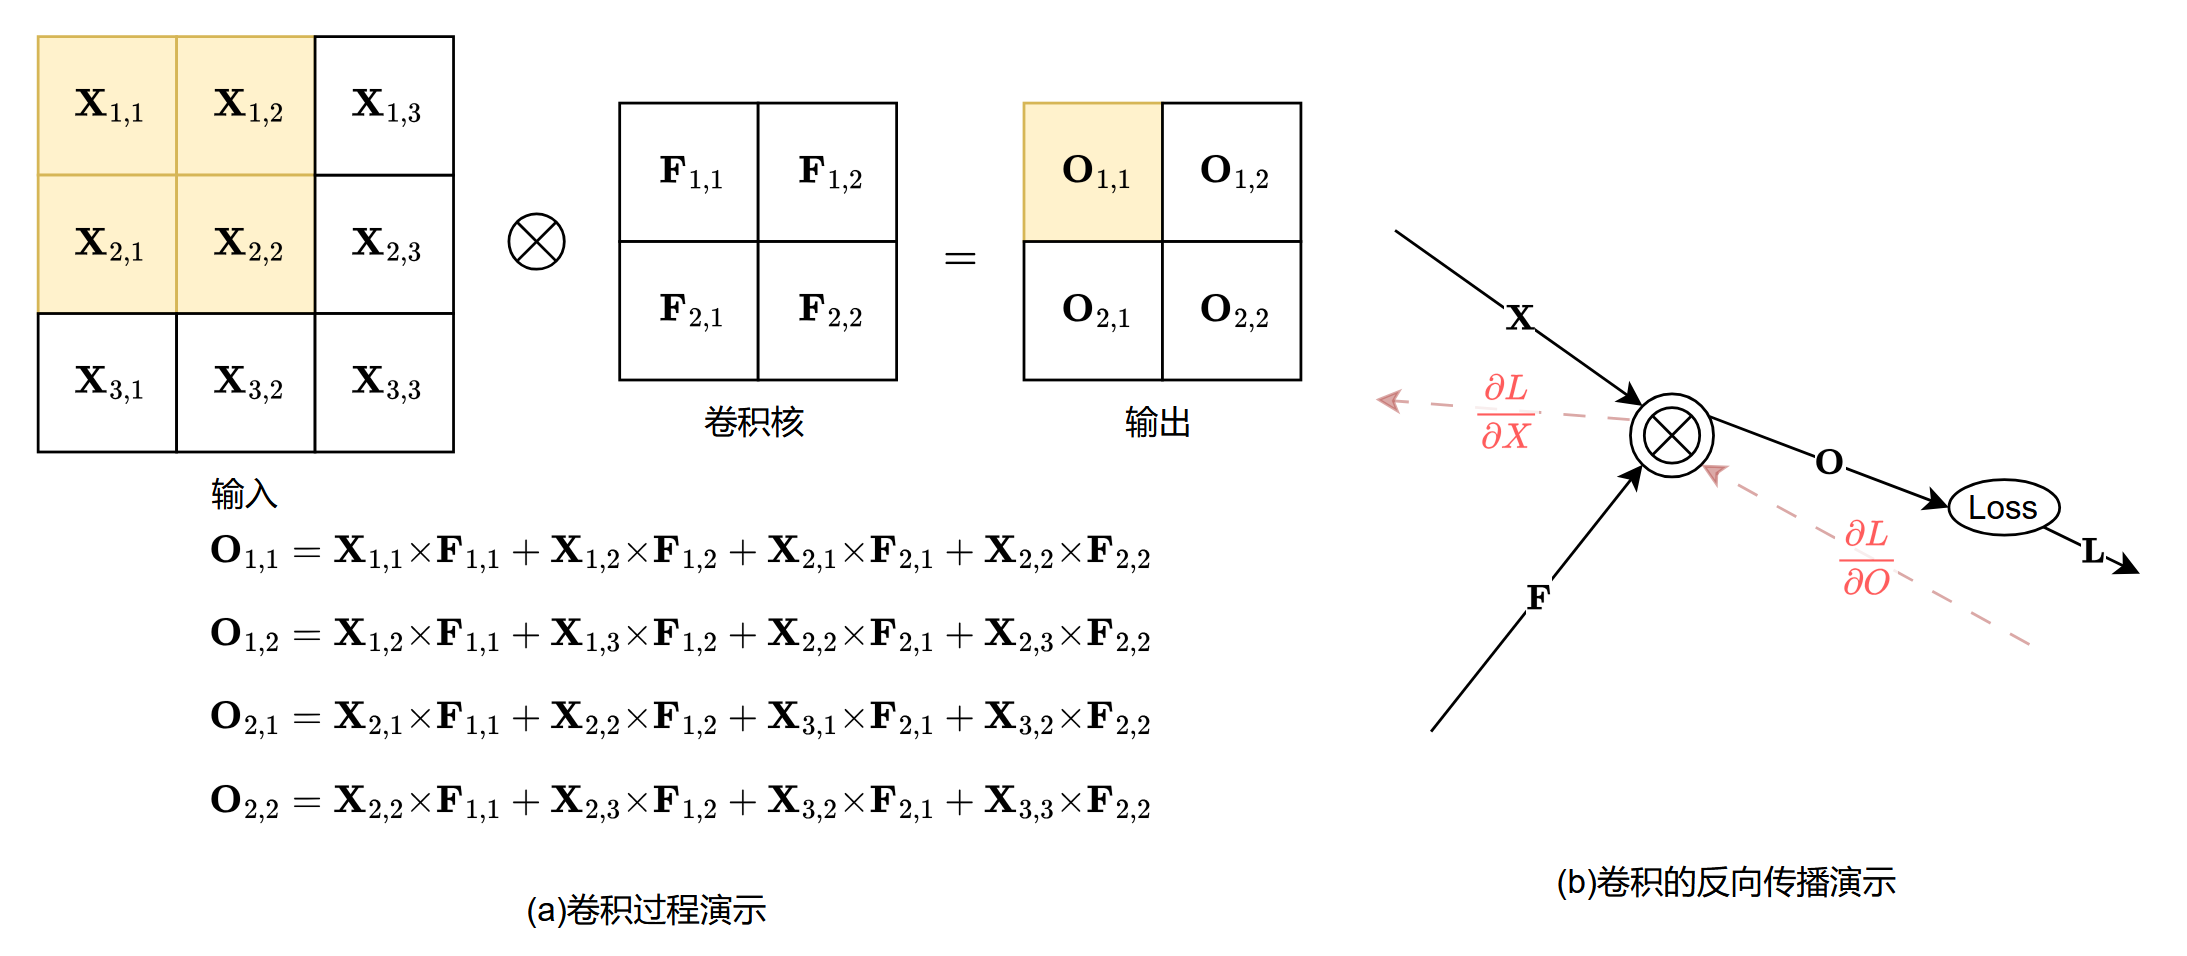
\includegraphics[scale=0.2]{conv.png}
			\label{figure}
		\end{figure}
		\item [(4)](5分)卷积是常用的数学运算,运算过程中,卷积核矩阵$\mathbf{F}$在输入矩阵$\mathbf{X}$上滑动,卷积核每滑动到与输入矩阵的某一子矩阵重叠时,卷积核与该子矩阵对应位置元素相乘再累加,得到输出结果在该位置的值。以步长(每次滑动的距离)等于1为例,其得到输出矩阵$\mathbf{O}$的过程和公式如图所示。
		


		已知,输入$\mathbf{X}=\begin{bmatrix}  
			3 & 1 & 2 \\  
			7 & 2 & 3 \\  
			4 & 5 & 6 \\
			
			\end{bmatrix}=(x_{ij})_{3 \times3},
			\ \text{卷积核}\ \mathbf{F}=\begin{bmatrix}  
			1 & -2 \\  
			-1 & 3 
			\end{bmatrix}=(f_{ij})_{2 \times2}$	
		
		根据卷积过程易得输出$\mathbf{O}=\begin{bmatrix}  
				0 & 4 \\  
				14 & 9  
				\end{bmatrix}$  ,${L}=Loss(\mathbf{O})$ 是关于 $\mathbf{O}$ 的某种损失函数。现在假设$\frac{{\partial}L}{{\partial}\mathbf{O}}=\begin{bmatrix}  
					3 & 7 \\  
					6 & 8    
					\end{bmatrix}$,请据此求解$\frac{{\partial}L}{{\partial}x_{11}}$ 和 $\frac{{\partial}L}{{\partial}\mathbf{X}}$	
		\end{itemize} 
\end{exercise}

\begin{Solution}
	(1)$\mathbf{X}\mathbf{X}^{-1}=\mathbf{I}$ 对两边同时作微分,有 $\mathbf{0}=d\mathbf{I}=d(\mathbf{X}\mathbf{X}^{-1})=d\mathbf{X} \mathbf{X}^{-1}+\mathbf{X}d(\mathbf{X}^{-1})$

整理可得 $d(\mathbf{X}^{-1})=-\mathbf{X}^{-1}d\mathbf{X} \mathbf{X}^{-1}$
\hfill \textcolor{red}{\textbf{(2分)}}

(2) 
$$
	\begin{aligned}
		dTr(\MX^\top \MX^{-1} \MA) &= Tr(d(\MX^\top \MX^{-1} \MA))\\
		&= Tr( d\MX^\top \MX^{-1}\MA -\MX^\top \MX^{-1} d\MX \MX^{-1} \MA)\\
		&= Tr((\MA^\top (\MX^{-1})^\top -\MX^{-1}\MA\MX^\top \MX^{-1}) d\MX)
	\end{aligned}
	$$
	
	即
	
	$$
	\begin{aligned}
		\frac{\partial Tr(\MX^\top \MX^{-1} \MA)}{\partial \MX} = (\MA^\top (\MX^{-1})^\top -\MX^{-1}\MA\MX^\top \MX^{-1})^\top
	\end{aligned}
	$$

	\hfill \textcolor{red}{\textbf{(5分)}}


(3) 先计算前项过程:

$A_1 x + b_1 
=
\begin{bmatrix}
4 \\
4 \\
-8
\end{bmatrix},
\text{ReLU}(A_1 x + b_1)=
\begin{bmatrix}
4 \\
4 \\
0
\end{bmatrix}
,
A_2 (\text{ReLU}(A_1 x + b_1)) + b_2 =
\begin{bmatrix}
1 \\
-1
\end{bmatrix}.$

$y=ReLU(A_2 (\text{ReLU}(A_1 x + b_1)) + b_2)=\begin{bmatrix}
	1 \\
	0
	\end{bmatrix},L = 1$

	\hfill \textcolor{red}{\textbf{(前向过程计算正确得3分)}}

	记:${k} = \text{ReLU}(A_1 x + b_1)$

	然后分别计算:
	$\frac{\partial L}{\partial {y}} =
	\begin{bmatrix}
	1 \\
	-1
	\end{bmatrix},
	\quad
	\frac{\partial {y}^T}{\partial {k}} =
	\begin{bmatrix}
	3 & 0 \\
	-1 & 0 \\
	0 & 0
	\end{bmatrix},
	\quad
	\frac{\partial {k}^T}{\partial b_1} =
	\begin{bmatrix}
	1 & 0 & 0 \\
	0 & 1 & 0 \\
	0 & 0 & 0
	\end{bmatrix}.$
	
	\hfill \textcolor{red}{\textbf{(三个矩阵各1分)}}

	所以有:

	$\frac{\partial L}{\partial b_1} =
	\frac{\partial {k}^T}{\partial b_1}
	\frac{\partial {y}^T}{\partial {k}}
	\frac{\partial L}{\partial {y}} =
	\begin{bmatrix}
	1 & 0 & 0 \\
	0 & 1 & 0 \\
	0 & 0 & 0
	\end{bmatrix}
	\begin{bmatrix}
	3 & 0 \\
	-1 & 0 \\
	0 & 0
	\end{bmatrix}
	\begin{bmatrix}
	1 \\
	-1
	\end{bmatrix}
	=
	\begin{bmatrix}
	3 \\
	-1 \\
	0
	\end{bmatrix}.$

	\hfill \textcolor{red}{\textbf{(写出最终结果1分)}}

	(3)根据链式法则,利用公式$\frac{{\partial}L}{{\partial}X_{ij}}=\underset{pq}{\sum} \frac{{\partial}O_{pq}}{{\partial}X_{ij}}\frac{{\partial}L}{{\partial}O_{pq}}$ 其中输出 $O_{pq}$ 和输入 $X_{ij}$ 有关联,$\frac{{\partial}O_{pq}}{{\partial}X_{ij}}$ 由卷积核$\mathbf{F}$具体的元素和 $X_{ij}$ 在 $\mathbf{F}$ 中的相对位置决定

	比如$\frac{{\partial}L}{{\partial}X_{11}}=\frac{{\partial}O_{11}}{{\partial}X_{11}}\frac{{\partial}L}{{\partial}O_{11}}$,$\frac{{\partial}L}{{\partial}X_{12}}=\frac{{\partial}O_{11}}{{\partial}X_{12}}\frac{{\partial}L}{{\partial}O_{11}}+\frac{{\partial}O_{12}}{{\partial}X_{12}}\frac{{\partial}L}{{\partial}O_{12}}$
	
	比如 $\frac{{\partial}O_{11}}{{\partial}X_{11}}=F_{11}=1$,$\frac{{\partial}O_{11}}{{\partial}X_{12}}=F_{12}=-2$,$\frac{{\partial}O_{12}}{{\partial}X_{12}}=F_{11}=1$
	
	同理,代入,可得:$\frac{{\partial}L}{{\partial}X}=\begin{bmatrix}  
		3 & 1 & -14  \\  
		3 & -2 & 5 \\  
		-6 & 10 & 24  \\
		\end{bmatrix}$

	\hfill \textcolor{red}{\textbf{(求得第一个元素得2分,求得完整的结果再得3分)}}
\end{Solution}


\begin{exercise}\quad(17分)
	\begin{itemize}
		\item [(1)](5分)判断函数$f(\mathbf{x}) = \max(\|\mathbf{A}\mathbf{x} + \mathbf{b}\|_2, \sqrt{{\mathbf{x}}^T \mathbf{x}} )+\frac{1}{2}{\mathbf{x}}^T\mathbf{P}\mathbf{x}$(其中$\mathbf{A} \in \mathbb{R}^{m \times n}, \, \mathbf{x} \in \mathbb{R}^n, \,\mathbf{b}  \in \mathbb{R}^m $,$\mathbf{P}$为$n$阶半正定矩阵) 是否为凸函数,并说明理由。
		\item [(2)](4分)考虑优化问题 $min f(\mathbf{x})=x_1^2+4x_1x_2$,从初始点$\mathbf{x}^{(0)}=(1,0)^T$出发,写出用梯度下降法迭代一步的过程,迭代时采用精确线搜索方法。
		\item [(3)](4分)利用二阶最优性条件找到问题 $minf(\mathbf{x})=x_1^2+4x_2^2+2x_1x_2$ 的全局最优解。
		\item [(4)](4分)证明 $f(\mathbf{x})=(\stackrel{n}{\underset{k=1}{\prod}}x_k)^{\frac{1}{n}}$,( $\mathbf{x}\in \mathbb{R}^{n}$且 $x_i>0$ ) 是凹函数。
		
		【提示,已知:\\ $\nabla f(\mathbf{x}) = \begin{pmatrix}
			\frac{f(\mathbf{x})}{n x_1}, \frac{f(\mathbf{x})}{n x_2}, \dots, \frac{f(\mathbf{x})}{n x_n}
			\end{pmatrix}^\top ,\quad\nabla^2 f(\mathbf{x}) =- \frac{f(\mathbf{x})}{n^2}
			\begin{bmatrix}
			\frac{n-1}{x_1^2} & -\frac{1}{x_1x_2} & \cdots & -\frac{1}{x_1x_n} \\
			-\frac{1}{x_2x_1} & \frac{n-1}{x_2^2} & \cdots & -\frac{1}{x_2x_n} \\
			\vdots & \vdots & \ddots & \vdots \\
			-\frac{1}{x_nx_1} & -\frac{1}{x_nx_2} & \cdots & \frac{n-1}{x_n^2}
			\end{bmatrix}.$】

	\end{itemize} 
\end{exercise}

\begin{Solution}
	(1)由仿射函数的任意范数为凸函数可知$\|Ax + b\|_2$为凸函数,另外$\sqrt{x^T x}$为$x$的2范数,显然为凸函数。根据逐点取最大值具有保凸性,可知$\max(\|Ax + b\|_2, \sqrt{x^T x} )$为凸函数。
	\hfill \textcolor{red}{\textbf{(3分)}}

	利用二阶条件,易得 $\frac{1}{2}x^TPx$ 也是凸函数
	\hfill \textcolor{red}{\textbf{(1分)}}
	
	由于凸函数相加具有保凸性,$f(x)$是凸函数。
	\hfill \textcolor{red}{\textbf{(1分)}}

	(2)$\nabla f(\mathbf{x}) = (2x_1+4x_2,4x_1)^T$

$-\nabla f(\mathbf{x}^{(0)}) =(-2,-4)^T$ 求解 $\lambda$:$\mathbf{x}^{(0)}-\lambda\nabla f(\mathbf{x}^{(0)})=(1-2\lambda,-4\lambda)^T$

$f(\mathbf{x}^{(0)}-\lambda\nabla f(\mathbf{x}^{(0)}))=36\lambda^2-20\lambda+1$ :$\lambda=\frac{-20}{-2 ×36}=\frac{5}{18}$ 时 $f(\mathbf{x}^{(0)}-\lambda\nabla f(\mathbf{x}^{(0)}))$最小

代入 $\lambda=\frac{5}{18}$ 可得 $\mathbf{x}^{(1)}=\mathbf{x}^{(0)}-\lambda\nabla f(\mathbf{x}^{(0)})=(\frac{4}{9},-\frac{10}{9})^T$

\hfill \textcolor{red}{\textbf{(4分)}}

(3)根据二阶最优性条件,我们需要使得下列式子同时成立,才能使得$\mathbf{x_1}$为全局最优解:
$\nabla f(\mathbf{x_1})=\mathbf{0},{\nabla }^2 f(\mathbf{x_1})\succ \mathbf{0}$
\hfill \textcolor{red}{\textbf{(两个式子各1分)}}

$f(\mathbf{x})=\mathbf{x}^T \begin{bmatrix}  
	1 & 1 \\  
	1 & 4  
	\end{bmatrix}\mathbf{x},\quad \nabla f(\mathbf{x})=\begin{bmatrix}  
	1 & 1 \\  
	1 & 4  
	\end{bmatrix}\mathbf{x},\quad {\nabla}^2 f(\mathbf{x})=\begin{bmatrix}  
	1 & 1 \\  
	1 & 4  
	\end{bmatrix}\succ \mathbf{0}$

	\hfill \textcolor{red}{\textbf{(1分)}}

	则只需使 $\nabla f(\mathbf{x_1})=\mathbf{0}=\begin{bmatrix}  
		1 & 1 \\  
		1 & 4  
		\end{bmatrix}\mathbf{x_1}$ 解得 $\mathbf{x_1}=\begin{bmatrix}  
		0 \\  
		0  
		\end{bmatrix}$ 这便是问题的全局最优解。

		\hfill \textcolor{red}{\textbf{(1分)}}

(4)要证 $f(\mathbf{x})$ 是凹函数,只需证 $\nabla^2  f(\mathbf{x})$ 半负定。

\hfill \textcolor{red}{\textbf{(1分)}}

根据提给条件


$\nabla^2  f(\mathbf{x}) = -\frac{ f(\mathbf{x})}{n^2}\begin{bmatrix}
	\frac{1}{x_1} & 0 & \cdots & 0 \\
	0 & \frac{1}{x_2} & \cdots & 0 \\
	\vdots & \vdots & \ddots & \vdots \\
	0 & 0 & \cdots & \frac{1}{x_n}
	\end{bmatrix}
	\begin{bmatrix}
	n-1 & -1 & \cdots & -1 \\
	-1 & n-1 & \cdots & -1 \\
	\vdots & \vdots & \ddots & \vdots \\
	-1 & -1 & \cdots & n-1
	\end{bmatrix}
	\begin{bmatrix}
	\frac{1}{x_1} & 0 & \cdots & 0 \\
	0 & \frac{1}{x_2} & \cdots & 0 \\
	\vdots & \vdots & \ddots & \vdots \\
	0 & 0 & \cdots & \frac{1}{x_n}
	\end{bmatrix}$


	$\begin{bmatrix}
		n-1 & -1 & \cdots & -1 \\
		-1 & n-1 & \cdots & -1 \\
		\vdots & \vdots & \ddots & \vdots \\
		-1 & -1 & \cdots & n-1
		\end{bmatrix}=nI_n-\begin{bmatrix}
		1 & 1 & \cdots & 1 \\
		1 & 1 & \cdots & 1 \\
		\vdots & \vdots & \ddots & \vdots \\
		1 & 1 & \cdots & 1
		\end{bmatrix}$
$I_n$特征值为1($n$重),$nI_n$特征值为$n$($n$重)

根据数学归纳法,
$\begin{bmatrix}
1 & 1 & \cdots & 1 \\
1 & 1 & \cdots & 1 \\
\vdots & \vdots & \ddots & \vdots \\
1 & 1 & \cdots & 1
\end{bmatrix}$特征值为$n$和0($n-1$重)

\hfill \textcolor{red}{\textbf{(3分)}}

故中间那个矩阵是实对称矩阵,且特征值为$n$($n-1$重)和0,是半正定矩阵,因此 $\nabla^2 f(x)$ 是半负定矩阵。
	

\end{Solution}


\end{document}